\documentclass[12pt, letterpaper]{article}
\usepackage[utf8]{inputenc}
\usepackage[english]{babel} % To obtain English text with the blindtext package
\usepackage{blindtext}
\usepackage{amsmath}
\usepackage{amssymb}
\usepackage{enumitem}
\usepackage{courier}
\usepackage{listings}
\usepackage{graphicx}
\usepackage{pgfplots}
\graphicspath{ {./images/} }

\lstdefinestyle{mystyle}{
    basicstyle=\fontsize{6}{8}\selectfont\ttfamily,
    breakatwhitespace=false,         
    breaklines=true,                 
    captionpos=b,                    
    keepspaces=true,                 
    numbers=left,                    
    numbersep=5pt,                  
    showspaces=false,                
    showstringspaces=false,
    showtabs=false,                  
    tabsize=2
}

\lstset{style=mystyle}

\title{CSCI2291 Homework 3}
\author{Jack Moffatt}
\date{February 3, 2022}


\begin{document}
\maketitle
\noindent\makebox[\linewidth]{\rule{18cm}{0.4pt}}

\section*{Problem 1}
\begin{enumerate}
    \item [(a)] We want to represent $\mu_r$ in terms of $\mu, \sigma^2, N,$ and $r$. 
        We can begin by defining $\mu$ as 
        \[
            \mu = \frac{\sum_{i=1}^Nx_i}{N}
        \]  
        It follows then that we can define $\mu_r$ after replacing the $r$ missing values with 
        $\mu$ as 
        \[
            \mu_r = \frac{\sum_{i=1}^Nx_i + r\mu}{N+r}
        \]
        Now, using our definition for $\mu$, we express $\mu_r$ and simplify
        \begin{align*}
            \frac{\sum_{i=1}^Nx_i + r\mu}{N+r} &= \frac{\sum_{i=1}^Nx_i + r(\frac{\sum_{i=1}^Nx_i}{N})}{N+r} \\
            &= \frac{(\frac{N(\sum_{i=1}^Nx_i)}{N}) + (\frac{r\sum_{i=1}^Nx_i}{N})}{N+r} \\
            &= \frac{(N+r)\sum_{i=1}^Nx_i}{N(N + r)} \\
            &= \frac{\sum_{i=1}^Nx_i}{N}
        \end{align*}
        So after some algebra we see that $\mu = \mu_r$.
    \item [(b)] Now, we want to follow similar steps to represent $\sigma_r^2$ in terms of $\mu, \sigma^2, N,$ and $r$. 
        We can again begin by defining $\sigma^2$ as 
        \[
            \sigma^2 = \frac{\sum_{i=1}^N(x_i - \mu)^2}{N-1}
        \]  
        It follows that we can then define $\sigma_r^2$ after replacing the $r$ missing values with 
        $\mu$ as 
        \[
            \sigma_r^2 = \frac{\sum_{i=1}^N(x_i - \mu)^2 + \sum_{i=N+1}^{N+r}(\mu - \mu)^2}{N+r-1}
        \]
        Now, since clearly evaluates to 0, as $\mu - \mu = 0$, we can use some algebra to see 
        \begin{align*}
            \sigma_r^2 &= \frac{\sum_{i=1}^N(x_i - \mu)^2 + \sum_{i=N+1}^{N+r}(\mu - \mu)^2}{N+r-1} \\
            \sigma_r^2 \cdot \frac{N+r-1}{N-1}&= \frac{\sum_{i=1}^N(x_i - \mu)^2}{N+r-1} \cdot \frac{N+r-1}{N-1}\\
            \sigma_r^2 \cdot \frac{N+r-1}{N-1}&= \sigma^2 \\
            \sigma_r^2 &= \sigma^2 \cdot \frac{N-1}{N+r-1}\\
        \end{align*}
        So we determine, since $\frac{N-1}{N+r-1} < 1$, that $\sigma_r^2 < \sigma^2$.
\end{enumerate}

\newpage
\noindent\makebox[\linewidth]{\rule{18cm}{0.4pt}}
\section*{Problem 2}
\begin{enumerate}
    \item [(a)] We will use the following code as a solution 
\begin{lstlisting}[language = python]
    from sklearn.manifold import MDS
    import matplotlib.pyplot as plt
    from sklearn import datasets
    
    breast_cancer = datasets.load_breast_cancer(as_frame = True)
    benign = breast_cancer.data.loc[breast_cancer.target == 0]
    malignant = breast_cancer.data.loc[breast_cancer.target == 1]
    
    projection = MDS(n_components = 2 )
    projected_benign = projection.fit_transform(benign)
    projected_malignant = projection.fit_transform(malignant)
    
    plt.scatter(projected_benign[:,0], projected_benign[:,1], c=['blue'])
    plt.scatter(projected_malignant[:,0], projected_malignant[:,1], c=['red'])
    plt.show()    
\end{lstlisting}
    We begin by loading the breast cancer data set from the datasets package of sklearn. By 
    setting the as frame parameter to True, we will receive our data formatted as a pandas DataFrame. 
    Then, we sort our data into two seperate DataFrame objects by sorting based on the target value, 
    which is benign and malignant. \\ \\ 
    Then, we can intialize our 2D projection, using the MDS module. And then we can transform each of our 
    datasets. Finally, using matplotlib we can make a scatter plot, with blue points for the benign dataset and 
    red points for the malignant dataset. The resulting scatter plot:
    \[
        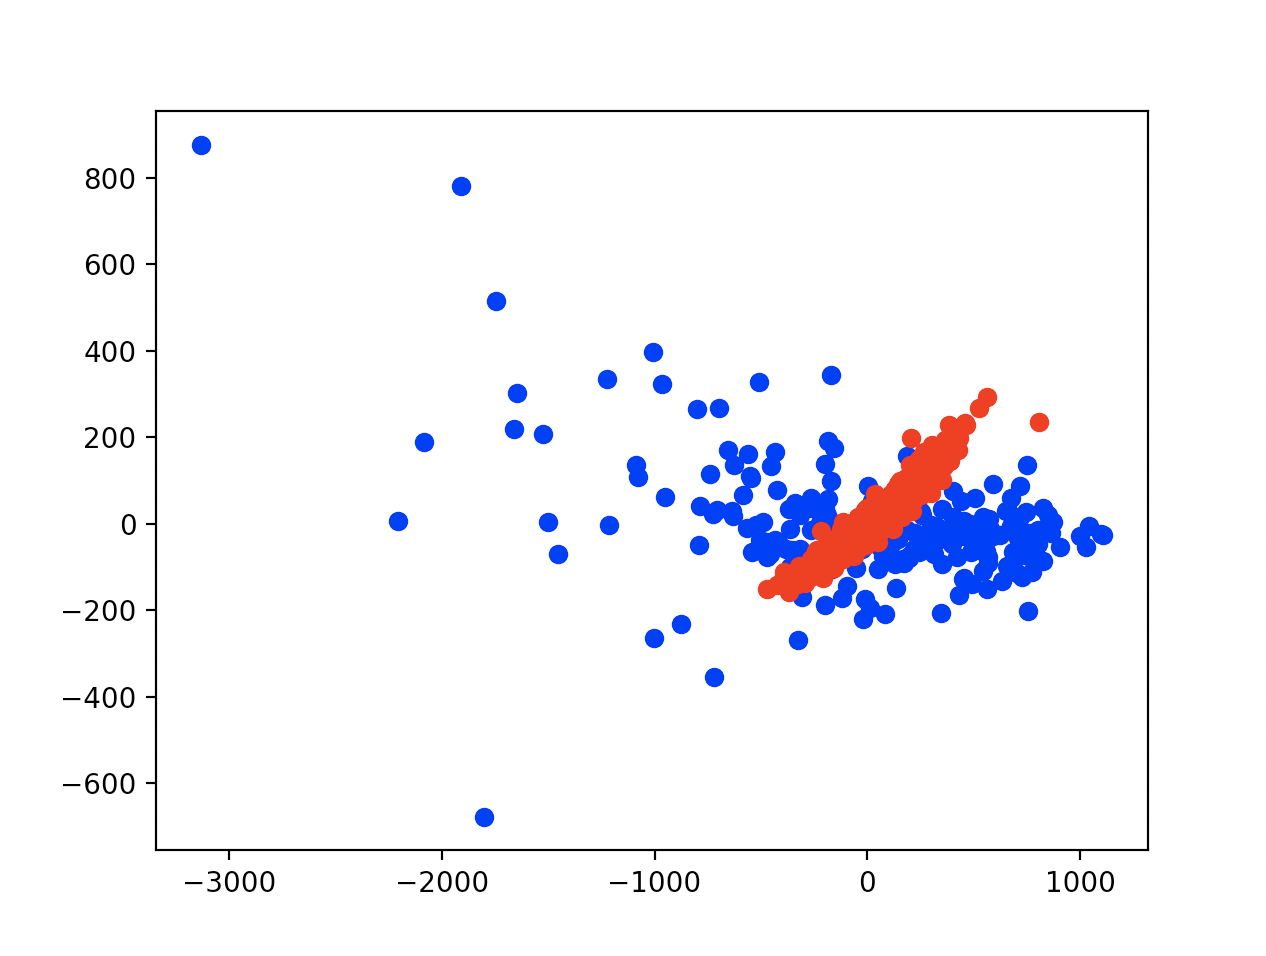
\includegraphics[scale=.33]{scatter_2a.png}
    \]  
    \item [(b)] We will use the following code as a solution
\begin{lstlisting}[language=python]
    from mpl_toolkits.mplot3d import Axes3D
    import matplotlib.pyplot as plt
    from sklearn.manifold import MDS
    from sklearn import datasets
    
    breast_cancer = datasets.load_breast_cancer(as_frame = True)
    benign = breast_cancer.data.loc[breast_cancer.target == 0]
    malignant = breast_cancer.data.loc[breast_cancer.target == 1]
    
    fig = plt.figure()
    ax = fig.add_subplot(111, projection = '3d')
    
    projection = MDS(n_components = 3)
    projected_benign = projection.fit_transform(benign)
    projected_malignant = projection.fit_transform(malignant)
    
    benign_scatter = ax.scatter(projected_benign[:,0], projected_benign[:,1], projected_benign[:,2], c=['blue'] )
    malignant_scatter = ax.scatter(projected_malignant[:,0], projected_malignant[:,1], projected_malignant[:,2], c=['red'] )
    plt.show()
\end{lstlisting}
    Lines 1-8 are identical to the solution in part {\bf a}. In lines 10 and 11 we intialize our 
    3D figure, following the guidelines provided in the documentation. \\ \\ 
    Again, we initialize our projection, except this time, we set the number of components to 3, 
    indicating we want a 3 dimensional projection. We then fit our projection onto each of our two 
    data sets. \\ \\ 
    Finally, using the figure we initialized in lines 10-11, we add scatter plots using the 3 columns of 
    our data sets as the X, Y, and Z axes. Again, our benign data points are colored blue, while malignant 
    data points are colored red. The resulting 3D scatter plot:
    \[
        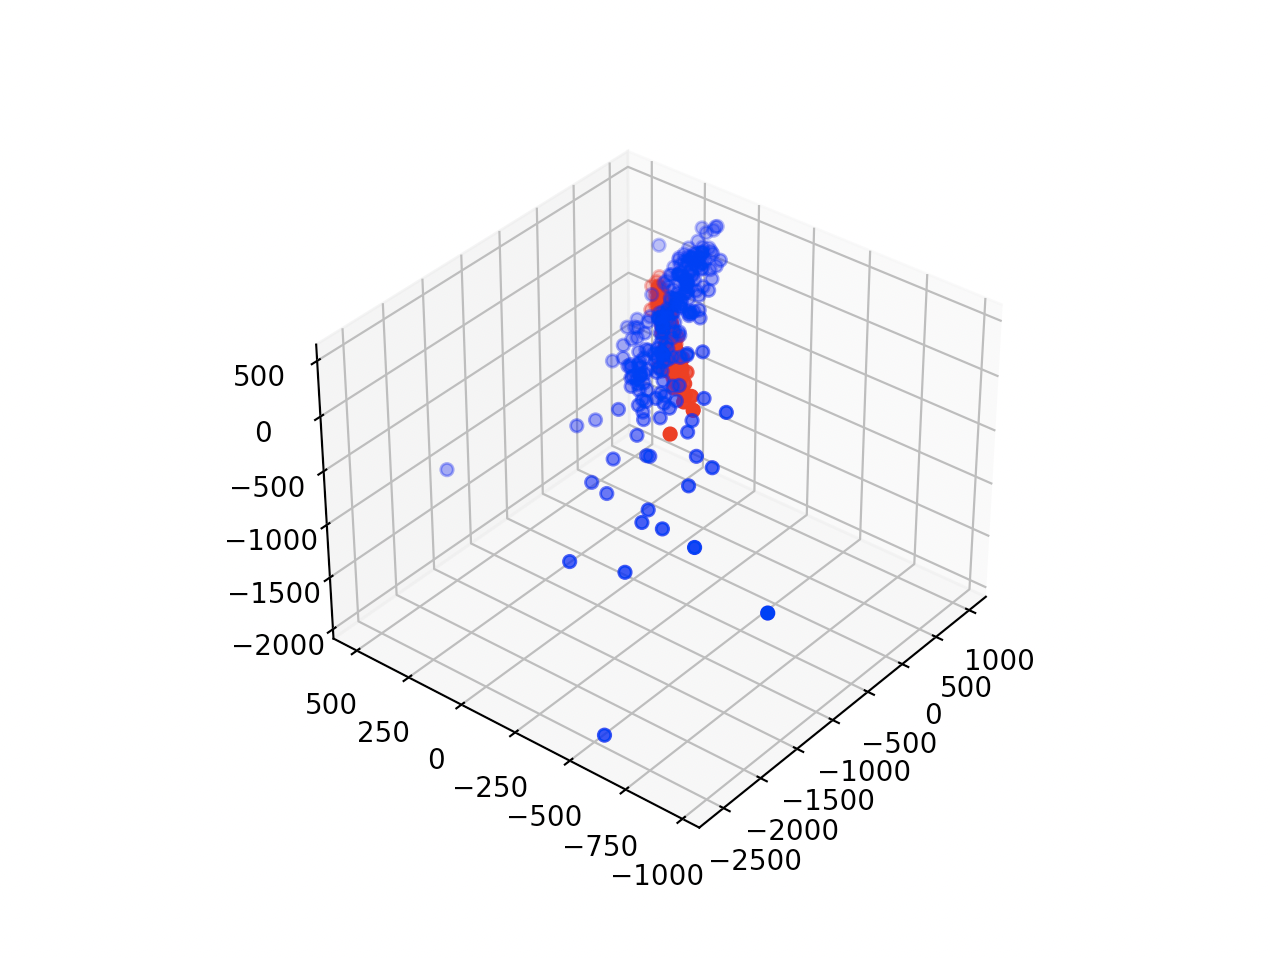
\includegraphics[scale=.33]{scatter_2b.png}
    \]
    
    \newpage
    \item [(c)] We will use the following code as a solution
\begin{lstlisting}[language=python]
    from sklearn import datasets
    from sklearn.manifold import MDS
    import matplotlib.pyplot as plt

    digits = datasets.load_digits(as_frame = True)
    projection = MDS(n_components = 2, )
    projected_digits = projection.fit_transform(digits.data)

    color_map = {
        '0' : 'red', '1' : 'blue',
        '2' : 'yellow', '3' : 'orange',
        '4' : 'maroon', '5' : 'green',
        '6' : 'saddlebrown', '7' : 'cyan',
        '8' : 'slategray', '9' : 'lime'
    }

    for target in digits.target_names:
        sorted_data = projected_digits[digits.target == target] 
        plt.scatter(sorted_data[:,0], sorted_data[:,1], c= [color_map[str(target)]] )
    plt.show()
\end{lstlisting}
    As in the first section of the problem, we load the digits data set and set as frame to True. Additionally, 
    we initialize an MDS projection to 2D space. Then we transform the digits data  to 2 dimensions. \\ \\
    As there are 10 target attributes, we set up a map to map each target name to a unique color to 
    use for our visualization. \\ \\
    Now we use a for loop to iterate over the target names, which for this particular dataset is a list of integers 
    between 0 and 9 inclusive. For each target value, we filter the projected data for only the 
    the points corresponding to the particular target value. Then, we add a scatter plot colored according to the color map. 
    After plotting the data for each target, we have the scatter plot: 
    \[
        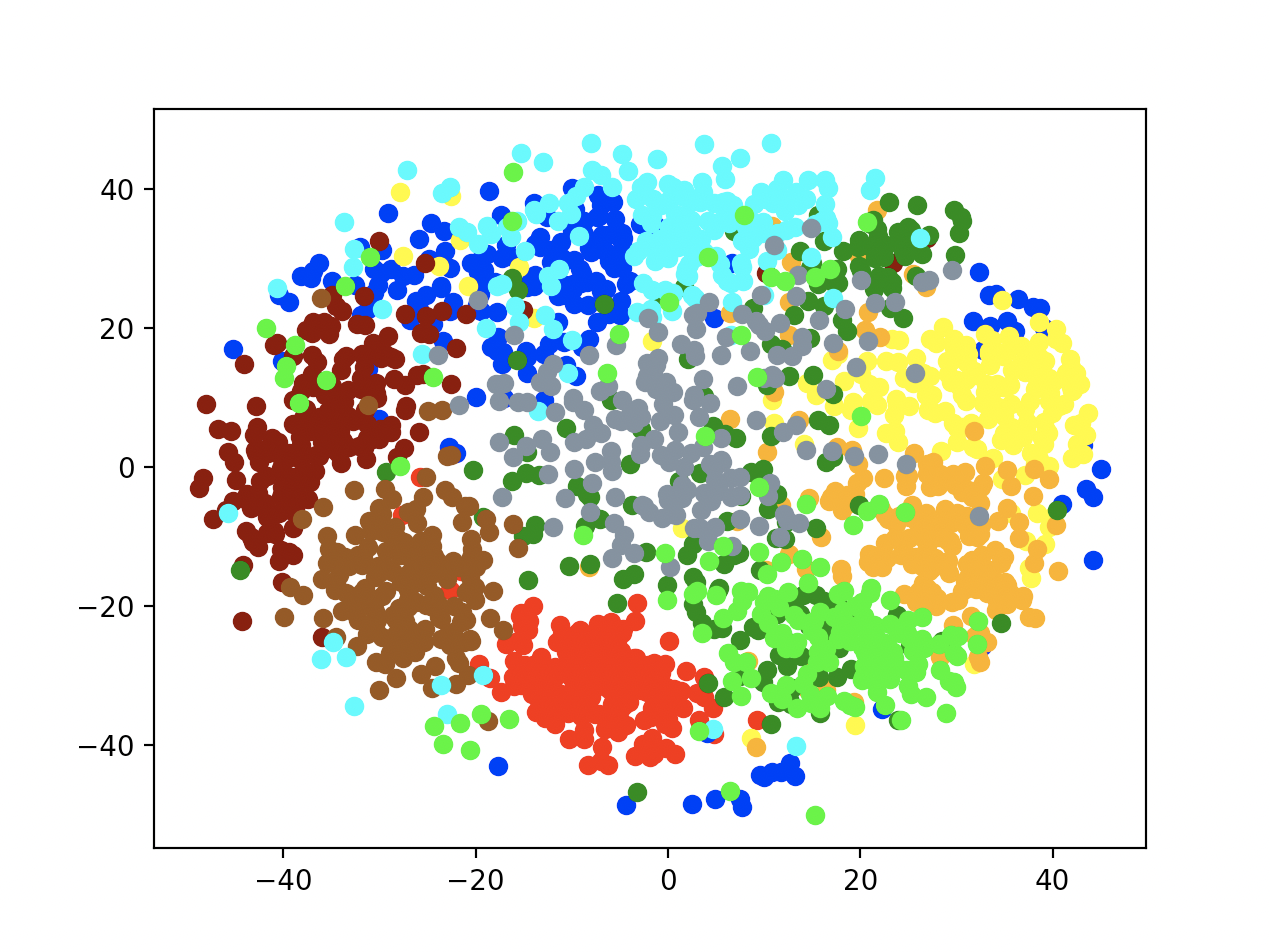
\includegraphics[scale=.33]{scatter_2c.png}
    \]  
    \item [(d)] We will use the following code for a solution: 
\begin{lstlisting}
    from mpl_toolkits.mplot3d import Axes3D
    import matplotlib.pyplot as plt
    from sklearn.manifold import MDS
    from sklearn import datasets
    
    digits = datasets.load_digits(as_frame = True)
    projection = MDS(n_components = 3, )
    projected_digits = projection.fit_transform(digits.data) 
    
    color_map = {
        '0' : 'red', '1' : 'blue',
        '2' : 'yellow', '3' : 'orange',
        '4' : 'maroon', '5' : 'green',
        '6' : 'saddlebrown', '7' : 'cyan',
        '8' : 'slategray', '9' : 'lime'
    }
    
    fig = plt.figure()
    ax = fig.add_subplot(111, projection = '3d')
    
    for target in digits.target_names:
        sorted_data = projected_digits[digits.target == target] 
        ax.scatter(sorted_data[:,0], sorted_data[:,1], sorted_data[:,2], c = [color_map[str(target)]] )
    plt.show()
\end{lstlisting}[language = python]
    Again, we load the data set, configure a 3D MDS projection and transform our data.
    Additionally, we can configure a color map to give unique colors for the data on each 
    of our target datasets. \\ \\ 
    Now, we can configure our 3D figure with the same lines that we did in part {\bf b}. Using the same 
    for loop as in part {\bf c} we create scatter plots for each target value. The only difference is now 
    we invoke a 3D scatter plot and pass the three columns of our projected data as the X, Y, and Z axes. 
    After plotting the data for each target, we have the scatter plot: 
    \[
        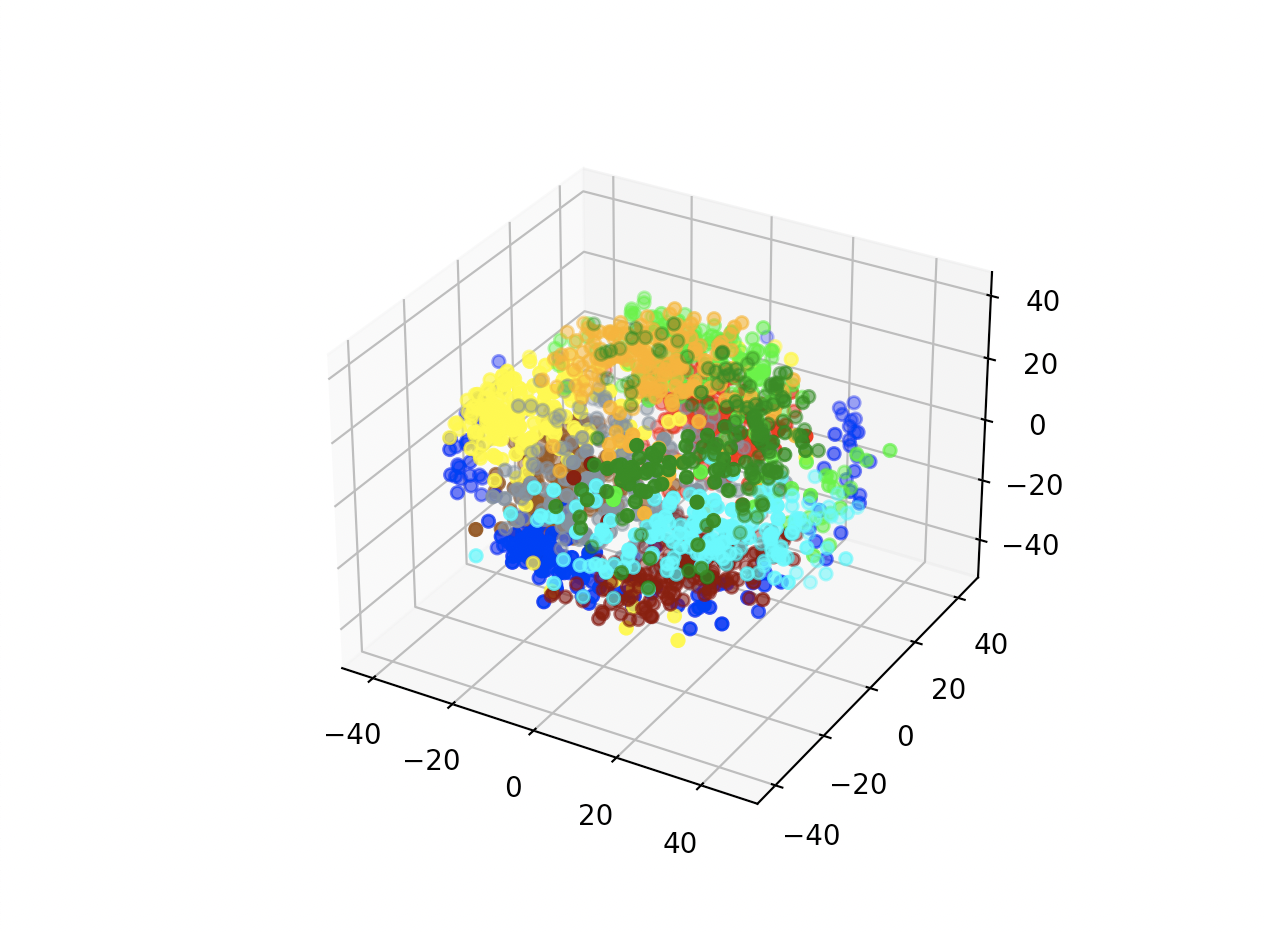
\includegraphics[scale = .33]{scatter_2d.png}
    \]  
\end{enumerate}

\newpage
\noindent\makebox[\linewidth]{\rule{18cm}{0.4pt}}
\section*{Problem 3}
\begin{enumerate}
    \item [(a)] We will use the following solution as our code
\begin{lstlisting}[language = python]
    import pandas as pd
    from matplotlib import pyplot as plt

    covid_variants = pd.read_csv("HW3/python/datasets/covid-variants.csv")
    us_variants = covid_variants.loc[covid_variants.location == "United States"]

    plt.boxplot([us_variants.num_sequences, us_variants.perc_sequences, us_variants.num_sequences_total])
    plt.show()
\end{lstlisting}
    We begin by importing pandas the pyplot package of matplotlib. Then, using the read csv function of 
    pandas, we read the covid variants data. Next we filter our data to get only the entries from 
    the United States. \\ \\ 
    Then we create a boxplot, using each of the descritive attributes in a list as the argument to plot 
    each box on a different index. We get the resulting scatter plot 
    \[
        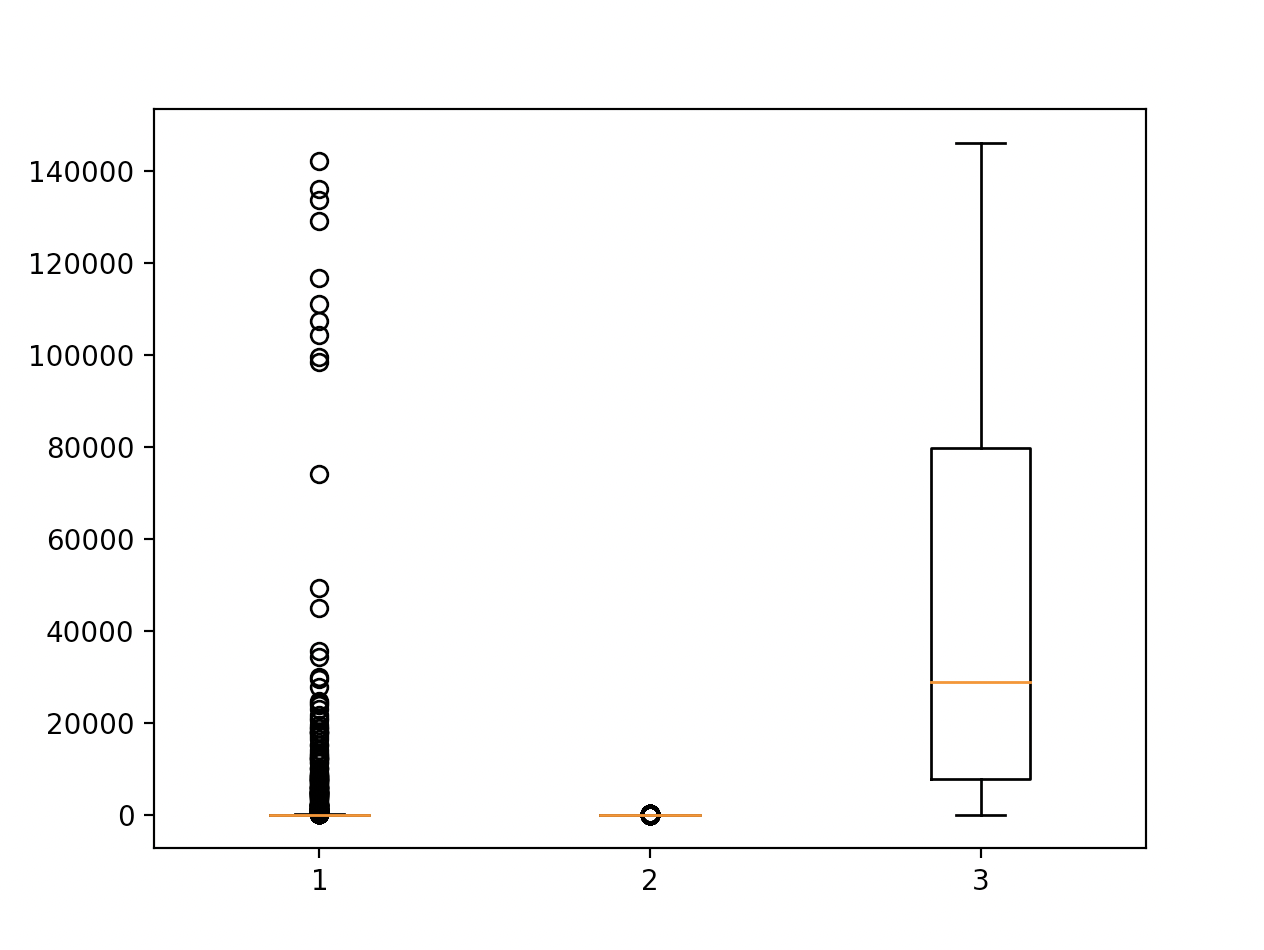
\includegraphics[scale = .33]{scatter_3a.png}
    \]  
    \newpage
    \item [(b)] We will use the following code as our solution:
\begin{lstlisting}[language = python]
    import pandas as pd

    covid_variants = pd.read_csv("HW3/python/datasets/covid-variants.csv")
    us_variants = covid_variants.loc[covid_variants.location == "United States"]
    weeks_list = us_variants.date.unique()

    count = 0

    for week in range(0, len(weeks_list)):
        if weeks_list[week][0:4] == '2021':
            num_sequences_total = us_variants.num_sequences_total.loc[us_variants.date == weeks_list[week]].mean()
            count += num_sequences_total

    print(f"Total number of US records in 2021: {int(count)}")
\end{lstlisting}
    Lines 1-5 are identical to part {\bf a}. Then we will additionally get a list 
    of the weeks that data samples were taken at by taking a unique indexed list of the 
    dates column of the data frame. \\ \\ 
    Then we will initialize a count and iterate over the list of dates and for 
    each date that occurs in 2021 we will take a count of the total number 
    of sequences in this week. Then we will increment this count by the numebr of 
    sequences. Upon running this code we get the output of 
\begin{lstlisting}[language = python]
    >>> Total number of US records in 2021: 1941782
\end{lstlisting}
\newpage
    \item [(c)] We will use the following code as our solution: 
\begin{lstlisting}[language=python]
    import pandas as pd

    covid_variants = pd.read_csv("HW3/python/datasets/covid-variants.csv")
    us_variants = covid_variants.loc[covid_variants.location == "United States"]
    canada_variants = covid_variants.loc[covid_variants.location == "Canada"]

    us_perc_sequences = us_variants.perc_sequences
    canada_perc_sequences = canada_variants.perc_sequences

    us_mean = us_perc_sequences.mean()
    canada_mean = canada_perc_sequences.mean()

    print(f"{'US Mean' :<15}{us_mean}")
    print(f"{'Canada Mean' :<15}{canada_mean}")
\end{lstlisting}
    Again we load our data and sort out the US data and we additionally sort 
    out the canadian data samples as well. Next, we seperate out the percentage of 
    sequences data attribute and then take the mean of each of these attribute values. 
    Printing our results we see
\begin{lstlisting}[language = python]
    >>> US Mean        6.239027777777777
    >>> Canada Mean    6.402651515151515
\end{lstlisting}
\newpage

    \item [(d)] We will use the following code as our solution:
\begin{lstlisting}[language = python]
    import pandas as pd
    import numpy as np
    import scipy.stats as stat
    
    covid_variants = pd.read_csv("HW3/python/datasets/covid-variants.csv")
    us_variants = covid_variants.loc[covid_variants.location == "United States"]
    canada_variants = covid_variants.loc[covid_variants.location == "Canada"]
    
    us_perc_sequences = us_variants.perc_sequences.to_numpy()
    canada_perc_sequences = canada_variants.perc_sequences.to_numpy()
    
    normalized_us =  (us_perc_sequences - np.mean(us_perc_sequences)) / np.std(us_perc_sequences)
    normalized_canada = (canada_perc_sequences - np.mean(canada_perc_sequences)) / np.std(canada_perc_sequences)
    
    t_test = stat.ttest_ind(normalized_us, normalized_canada)
    
    print(t_test)
\end{lstlisting}
    Lines 5-10 are identical to part {\bf c}, however this time we convert the percentage of 
    sequences into NumPy arrays. Next, we normalize our data so that we can apply a t test to the data. \\ \\ 
    We select the independent t test because our samples come from separate populations, so there 
    is no relationship between the two datasets. Passing our two normalized attribute value vectors 
    to the t test we receive both a t value (statistic) and a p value which is a measure of our interval 
    of confidence. Running the print statement, we get the values 
\begin{lstlisting}[language = python]
    >>> Ttest_indResult(statistic=-7.839338635406006e-16, pvalue=0.9999999999999993)
\end{lstlisting}
    We can see that our t value is 0 and since our p value is essentially 1, we have a very high interval of connfidence. This tells 
    us that the difference in the sample means is incredibly likely to occur in the respective populations as well. 
\end{enumerate}

\newpage
\noindent\makebox[\linewidth]{\rule{18cm}{0.4pt}}
\section*{Problem 4}
Our group currently consists of myself, Alexander Benati, Bryan Kim, and Ayush Patel. We are currently 
planning on working on a music recommendation system based on Spotify music data. 



\end{document}